\chapter{Conjugate Gradients}
The conjugate gradient iteration is the "original" Krylov subspace iteration, the most famous of these methods and one of the mainstays of scientific computing. Discovered by Hestenes and Stiefel in 1952, it solves symmetric positive definite systems of equations amazingly quickly if the eigenvalues are well distributed.

\section{Minimizing the 2-Norm of the Residual} 
 We have learned about GMRES. At step $ n $, $ x_* $ is approximated by the vector $ x_n \in \cK_n $ that minimizes $ \|r_n\|_2 $, where $ r_n = b-Ax $. Since $ A $ is symmetric, faster algorithms are available based on three-term instead of $ (n+1) $-term recurrences at step $ n $. One of these goes by the names of conjugate residuals or MINRES(``minimal residuals'').  

 \section{Minimizing the $ A $-Norm of the Error} 
 Assume $ A $ is also positive definite. Then we can define $ A $ norm by 
 \[
    \|x\|_A = \sqrt{x^\top Ax} . 
 \]
Now we care about the vector $ e_n = x_* x_n $. The conjugate gradient iteration can be described as follows. \textbf{It is a system of recurrence formulas that generates the unique sequence of iterates $ \{x_n \in \cK_n\}  $ with the property that at step $ n $, $ \|e_n\|_A $ is minimized.}


\section{The Conjugate Gradient Iteration} 
\begin{algorithm}[H]
    \caption{Conjugate Gradient (CG) Iteration}
    \label{Algo 38.1}
    $ x_0=0, r_0=b, p_0=r_0 $\;
    \For {$ n=1,2,3,\ldots  $}{
        $ \alpha _n = (r_{n-1}^\top r_{n-1}) / (p_{n-1}^\top A P_{n-1}) $ \tcp*{ step length } 
        $ x_n = x_{n-1} + \alpha _n p_{n-1} $ \tcp*{ approximate solution } 
        $ r_n = r_{n-1} - \alpha _n A p_{n-1} $ \tcp*{ residual } 
        $ \beta _n = (r_n^\top r_n) /(r_{n-1}^\top r_{n-1}) $ \tcp*{ improvement this step } 
        $ p_n = r_{n} + \beta _n p_{n-1}  $ \tcp*{ search direction } 
    }
\end{algorithm}

Before analyzing the mathematical properties of these formulas, let us examine them operationally. The algorithm is extraordinarily simple. The only complication-which we shall not address—is the choice of a convergence criterion.

From the five lines that define the algorithm, the following properties can be deduced. Like all the theorems in this book that do not explicitly mention rounding errors, this one assumes that the computation is performed in exact arithmetic. If there are rounding errors, these properties fail, and it becomes a subtle matter to explain the still very impressive performance of CG.


%────────────────────────────────────────
\begin{theorem}
[Properties of CG]
\label{thm: Properties of CG}
Let the CG  iteration (\autoref{Algo 37.1}) be applied to a symmetric positive definite matrix problem $ Ax=b $. As long as the iteration has not yet converged, the algorithm proceeds without divisions by zero, and we have the following identities of subspaces: 
\begin{equation}
\label{eq: subspaces of CG}
    \begin{aligned}
        \cK_n &= \langle x_1,x_2,\ldots ,x_n \rangle  = \langle p_0, p_1,\ldots ,p_{n-1} \rangle  \\ 
        &= \langle r_0, r_1,\ldots r_{n-1} \rangle  = \langle b, Ab ,\ldots ,A^{n-1}b \rangle . 
    \end{aligned}
\end{equation}
Moreover, the residuals are orthogonal, 
\begin{equation}
\label{eq: CG orthogonal res}
    r_n^\top r_j = 0, \quad \forall j < n, 
\end{equation}
and the search direction are ``A-conjugate,''
\begin{equation}
\label{eq: A-conjugate CG}
    p_n^\top Ap_j = 0, \quad \forall j< n. 
\end{equation}
\end{theorem}
%────────────────────────────────────────
%────────────────────────────────────────
\begin{proof}[Proof sketch]
We can prove all these by induction. 
\end{proof}
%────────────────────────────────────────

\section{Optimality of CG} 
 

%────────────────────────────────────────
\begin{theorem}
[Optimality of CG]
\label{thm: Optimality of CG}
Let the CG iteration be applied to a symmetric positive definite matrix problem $ Ax=b $. If the iteration has not already converged (i.e., $ r_{n-1}\neq 0 $), then $ x_n $ is the unique point in $ \cK_n $ that minimizes $ \|e_n\|_A $. The convergence is monotonic, 
\begin{equation}
\label{eq: optimality of CG}
    \|e_n \|_A \le \|e_{n-1}\|_A,
\end{equation}
and $ e_n = 0 $ is achieved for some $ n\le m $. 
\end{theorem}
%────────────────────────────────────────

%────────────────────────────────────────
\begin{proof}
From Thm~\ref{thm: Properties of CG}, we know that $ x_n $ belongs to $ \cK_n $. Proof.  To show that it is the unique point in $\mathcal{K}_n$ that minimizes $\|e\|_A$, consider an arbitrary point $x=x_n-\Delta x \in \mathcal{K}_n$, with error $e=x_*-x=e_n+\Delta x$. We calculate
$$
\begin{aligned}
\|e\|_A^2 & =\left(e_n+\Delta x\right)^T A\left(e_n+\Delta x\right) \\
& =e_n^T A e_n+(\Delta x)^T A(\Delta x)+2 e_n^T A(\Delta x) .
\end{aligned}
$$
The final term in this equation is $2 r_n^T(\Delta x)$, an inner product of $r_n$ with a vector in $\mathcal{K}_n$, and by Thm~\ref{thm: Properties of CG} any such inner product is zero. This is the crucial orthogonality property that makes the CG iteration so powerful. It implies that we have
$$
\|e\|_A^2=e_n^T A e_n+(\Delta x)^T A(\Delta x)
$$
Only the second of these terms depends on $\Delta x$, and since $A$ is positive definite, that term is $\geq 0$, attaining the value 0 if and only if $\Delta x=0$, i.e., $x_n=x$. Thus $\|e\|_A$ is minimal if and only if $x_n=x$, as claimed.

The remaining statements of the theorem now follow readily. The monotonicity property \eqref{eq: optimality of CG} is a consequence of the inclusion $\mathcal{K}_n \subseteq \mathcal{K}_{n+1}$, and since $\mathcal{K}_n$ is a subset of $\mathbb{R}^m$ of dimension $n$ as long as convergence has not yet been achieved, convergence must be achieved in at most $m$ steps.
\end{proof}
%────────────────────────────────────────
The guarantee that the CG iteration converges in at most $m$ steps is void in floating point arithmetic. For arbitrary matrices $A$ on a real computer, no decisive reduction in $\left\|e_n\right\|_A$ will necessarily be observed at all when $n=m$. In practice, however, CG is used not for arbitrary matrices but for matrices whose spectra, perhaps thanks to preconditioning, are well-enough behaved that convergence to a desired accuracy is achieved for $n \ll m$.

\section{CG as an Optimization Algorithm} 
We have just shown that the CG iteration has a certain optimality property: it minimizes $\left\|e_n\right\|_A$ at step $n$ over all vectors $x \in \mathcal{K}_n$. In fact, as foreshadowed already by the use of such terms as ``step length'' and ``search direction,'' this iteration can be interpreted as an algorithm of a standard form for minimizing a nonlinear function of $x \in \mathbb{R}^m$. At the heart of the iteration is the formula
$$
x_n=x_{n-1}+\alpha_n p_{n-1} \text {. }
$$
This is a familiar equation in optimization, in which a current approximation $x_{n-1}$ is updated to a new approximation $x_n$ by moving a distance $\alpha_n$ (the step length) in the direction $p_{n-1}$ (the search direction). By a succession of such steps, the CG iteration attempts to find a minimum of a nonlinear function.

In fact, this function is 
\begin{equation}
\label{eq: CG optimize function}
    \varphi(x) = \frac{1}{2}x^\top Ax  - x^\top b. 
\end{equation}
In fact, a short computation now reveals 
\[
    \begin{aligned}
        \left\|e_n\right\|_A^2 & =e_n^T A e_n=\left(x_*-x_n\right)^T A\left(x_*-x_n\right) \\
        & =x_n^T A x_n-2 x_n^T A x_*+x_*^T A x_* \\
        & =x_n^T A x_n-2 x_n^T b+x_*^T b=2 \varphi\left(x_n\right)+\text { constant. }
        \end{aligned}
\]
Thus $ \varphi(x) $ is the same as $ \|e\|_A^{2} $ except for a factor of $ 2 $ and the constant $ x_*^\top b $. This function must achieve its minimum uniquely at $ x=x_* $.  

At each step, an iterate $ x_n = x_{n-1} + \alpha _n p_{n-1} $ is computed that minimize $ \varphi(x) $ over all $ x $ in the one-dimensional space $ x_{n-1}+ \langle p_{n-1} \rangle $. What makes the CG iteration remarkable is the choice of the search direction $ p_{n-1} $, which has the special property that minimizing $ \varphi(x) $ over $ x_n + \langle p_{n-1} \rangle  $ actually minimizes it over all of $ \cK_n $. 

There is a close analogy between the CG iteration for solving $A x=b$ and the Lanczos iteration for finding eigenvalues. The eigenvalues of $A$, as discussed in Chapter 26, are the stationary values for $x \in \mathbb{R}^m$ of the Rayleigh quotient, $r(x)=\left(x^T A x\right) /\left(x^T x\right)$. The eigenvalue estimates (Ritz values) associated with step $n$ of the Lanczos iteration are the stationary values of the same function $r(x)$ if $x$ is restricted to the Krylov subspace $\mathcal{K}_n$. This is a perfect parallel of what we have shown in the last two pages, that the solution $x_*$ of $A x=b$ is the minimal point in $\mathbb{R}^m$ of the scalar function $\varphi(x)$, and the CG iterate $x_n$ is the minimal point of the same function $\varphi(x)$ if $x$ is restricted to $\mathcal{K}_n$.

\section{CG and Polynomial Approximation} 
For the CG, the approximation problem is: 


%────────────────────────────────────────
\begin{example}
[CG Approximation problem]
\label{eg: CG Approximation problem}
\[
    \arg \min_{p_n \in P_n} \|p_n(A) e_0\|_A. 
\]
Here $ e_0 = x_* -x_0 = x_* $ and $ P_n = \{p\in \RR[x]| \deg(p)\le n , p(0) =1\}  $. 
\end{example}
%────────────────────────────────────────

We have the following convergence theorem. 

%────────────────────────────────────────
\begin{theorem}
\label{thm: Convergence of CG}
If the CG iteration has not already converged before step $n$ (i.e., $r_{n-1} \neq 0$ ), then the CG approximation problem has a unique solution $p_n \in P_n$, and the iterate $x_n$ has error $e_n=p_n(A) e_0$ for this same polynomial $p_n$. Consequently we have
$$
\frac{\left\|e_n\right\|_A}{\left\|e_0\right\|_A}=\inf _{p \in P_n} \frac{\left\|p(A) e_0\right\|_A}{\left\|e_0\right\|_A} \leq \inf _{p \in P_n} \max _{\lambda \in \Lambda(A)}|p(\lambda)|
$$
where $\Lambda(A)$ denotes the spectrum of $A$.
\end{theorem}
%────────────────────────────────────────

\section{Rate of Convergence} 
Thm~\ref{thm: Convergence of CG} establishes that the rate of convergence of the CG iteration is determined by the location of the spectrum of $ A $.  A good spectrum is one on which polynomials $p_n \in P_n$ can be very small, with size decreasing rapidly with $n$. Roughly speaking, this may happen for either or both of two reasons: the eigenvalues may be grouped in small clusters, or they may lie well separated in a relative sense from the origin. 
 
First, we suppose the eigenvalues are perfectly clustered. 

%────────────────────────────────────────
\begin{corollary}
\label{cor: CG distinct eig}
If $ A $ has only $ n $ distinct eigenvalues, then the CG iteration converges in at most $ n $ steps. 
\end{corollary}
%────────────────────────────────────────

At the other extreme, suppose we know nothing about any clustering of the eigenvalues but only that heir distances from the origin vary by at most a factor $ \kappa \ge 1 $. $ \kappa = \lambda _{\max} /  \lambda _{ \min }$. 


%────────────────────────────────────────
\begin{corollary}
\label{cor: CG size of eig }
Let the CG iteration be applied to a symmetric positive definite matrix problem $A x=b$, where $A$ has 2-norm condition number $\kappa$. Then the A-norms of the errors satisfy
$$
\frac{\left\|e_n\right\|_A}{\left\|e_0\right\|_A} \leq 2 /\left[\left(\frac{\sqrt{\kappa}+1}{\sqrt{\kappa}-1}\right)^n+\left(\frac{\sqrt{\kappa}+1}{\sqrt{\kappa}-1}\right)^{-n}\right] \leq 2\left(\frac{\sqrt{\kappa}-1}{\sqrt{\kappa}+1}\right)^n. 
$$
\end{corollary}
%────────────────────────────────────────
%────────────────────────────────────────
\begin{proof}[Proof sketch]
Consider the shifted Chebyshev polynomial 
\[
    p(x) = \frac{T_n\left (\gamma  - \frac{2x}{\lambda_{\max} - \lambda _{\min}}\right )}{T_n(\gamma )},
\]
where $ \gamma  $ takes the special value $ \gamma = \frac{\lambda _{\max} + \lambda _{\min}}{\lambda _{\max}-\lambda _{\min}} = \frac{\kappa+1}{\kappa-1} $. For $ x\in [\lambda _{\min}, \lambda _{\max}] $, the argument of $ T_n $ in the numerator of $ p(x) $ lies in $ [-1,1] $, which means the magnitude of that numerator is $ \le 1 $. Therefore, we only need to show 
\[
    T_n(\gamma)=T_n\left(\frac{\kappa+1}{\kappa-1}\right)=\frac{1}{2}\left[\left(\frac{\sqrt{\kappa}+1}{\sqrt{\kappa}-1}\right)^n+\left(\frac{\sqrt{\kappa}+1}{\sqrt{\kappa}-1}\right)^{-n}\right] .
\]
Since we know if $ x= \frac{1}{2}(z + z^{-1} ), T_n(x) = \frac{1}{2}(z^{n} + z^{-n}) $, we can show this with a change of variable.  
\end{proof}
%────────────────────────────────────────

Corollary~\ref{cor: CG size of eig } is the most famous result about convergence of the CG iteration. Since
$$
\frac{\sqrt{\kappa}-1}{\sqrt{\kappa}+1} \sim 1-\frac{2}{\sqrt{\kappa}}
$$
as $\kappa \rightarrow \infty$, it implies that if $\kappa$ is large but not too large, convergence to a specified tolerance can be expected in $O(\sqrt{\kappa})$ iterations. One must remember that this is only an upper bound. Convergence may be faster for special righthand sides (not so common) or if the spectrum is clustered (more common).

\section{Example} 
For an example of the convergence of CG, consider a $500 \times 500$ sparse matrix $A$ constructed as follows. First we put 1 at each diagonal position and a random number from the uniform distribution on $[-1,1]$ at each off-diagonal position (maintaining the symmetry $A=A^T$ ). Then we replace each off-diagonal entry with $\left|a_{i j}\right|>\tau$ by zero, where $\tau$ is a parameter. For $\tau$ close to zero, the result is a well-conditioned positive definite matrix whose density of nonzero entries is approximately $\tau$. As $\tau$ increases, both the condition number and the sparsity deteriorate. 

%────────────────────────────────────────
\begin{figure}[H]
    \centering
    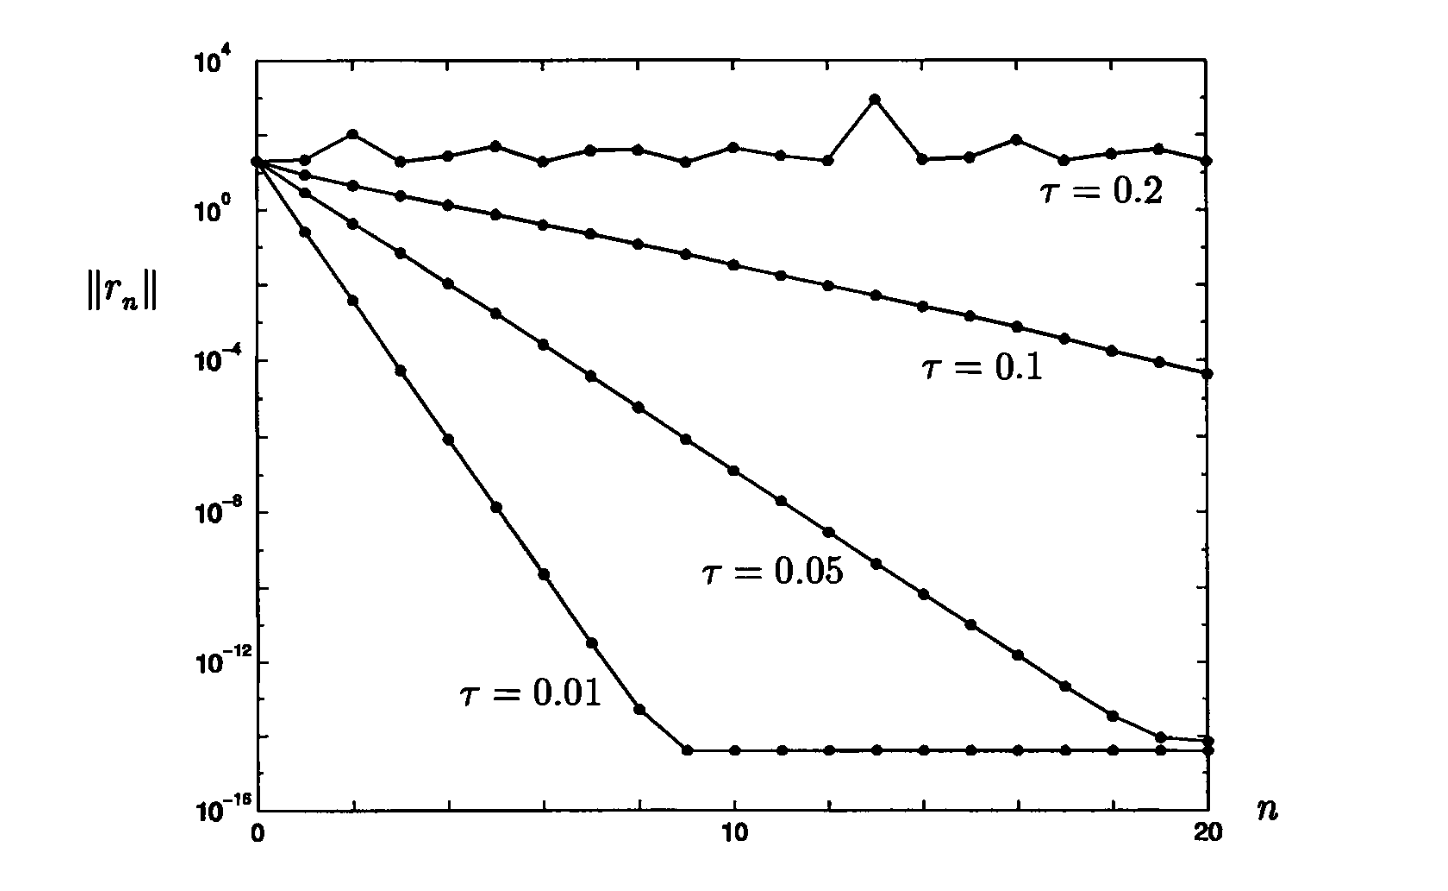
\includegraphics[width=0.8\textwidth]{figures/38-1.png}
    \caption{CG convergence curves for the $500 \times 500$ sparse matrices $A$ described in the text. For $\tau=0.01$, the system is solved about 700 times faster by $C G$ than by Cholesky factorization. For $\tau=0.2$, the matrix is not positive definite and there is no convergence.}
\end{figure}
%────────────────────────────────────────

Note that for $\tau=0.2$, with 50,834 nonzeros, there is no convergence at all. The lowest eigenvalue is now negative, so $A$ is no longer positive definite and the use of the CG iteration is inappropriate. (In fact, the CG iteration often succeeds with indefinite matrices, but in this case the matrix is not only indefinite but ill-conditioned.)

When $ \tau=0.01 $, the operation count of $6 \times 10^4$ flops beats Cholesky factorization (23.4) by a factor of about 700. Unfortunately, not every matrix arising in practice has such a well-behaved spectrum, even after the best efforts to find a good preconditioner.